\section{Experiment}
In this chapter we describe the experiments conducted on heartbeat data taken from the MIT-BIH Arrhythmia data set. Afterwards we present the results and draw insights. The aim is to assess the utility of synthetic data generated by the two algorithms mentioned in \cref{chapter4}. The utility is measured in the downstream task of arrhythmia detection. We are testing differentially private and non-private versions of the models and compare them to a baseline model that is trained on the original data.

\subsection{Data Set and Experiment setup}
The MIT-BIH is a commonly used benchmark data set for arrhythmia detection. It contains two channel ECG data collected in the 1980s from some 47 patients by the Arrhythmia Laboratory of Boston's Beth Israel Hospital (BIH; now the Beth Israel Deaconess Medical Center). 23 patients were chosen at random from a pool of over 4000 thousand patients, whereas the rest was chosen to include examples of clinically important but statistically uncommon arrhythmias. Hence, the proportion of arrhythmias in the whole data set is much larger than in reality. Studies suggest a percentage between 1.5\% and 5\% of patients with arrhythmias depending on the reference group \parencite{desai2022arrhythmias}. 

\begin{figure}[h]
    \centering
    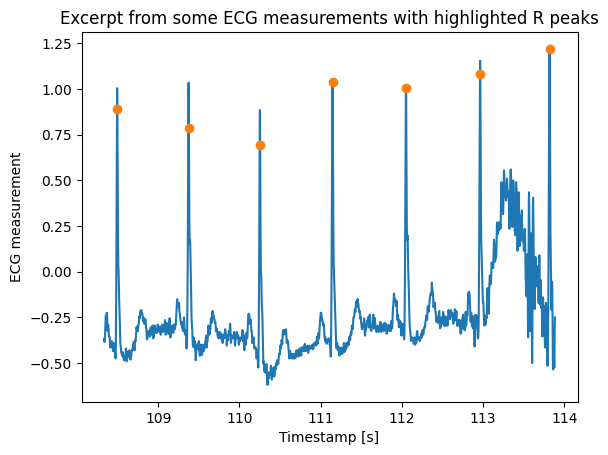
\includegraphics[scale=0.7]{excerpt_ecg_rpeaks.png}
    \caption{Excerpt from one ECG data sample, where the R peaks are highlighted}
\end{figure}

One single, regular heartbeat consists of one so-called QRS complex that consists of three blocks: a Q wave, R wave and S wave. Heartbeat arrhythmia is a medical condition in which the patient experiences an abnormal rhythm of heartbeat. In most cases, this can be diagnosed by looking at the ECG: abnormal shapes in the different blocks or duration can indicate arrhythmia. This can be treated as an anomaly detection problem, where we train a model to learn the probability distribution of regular heartbeats (e. g. to capture their shape characteristics in terms of the building blocks). Based on some decision rule the model can detect samples that come from this distribution or were sampled from a different distribution.

\begin{figure}[h]
    \centering
    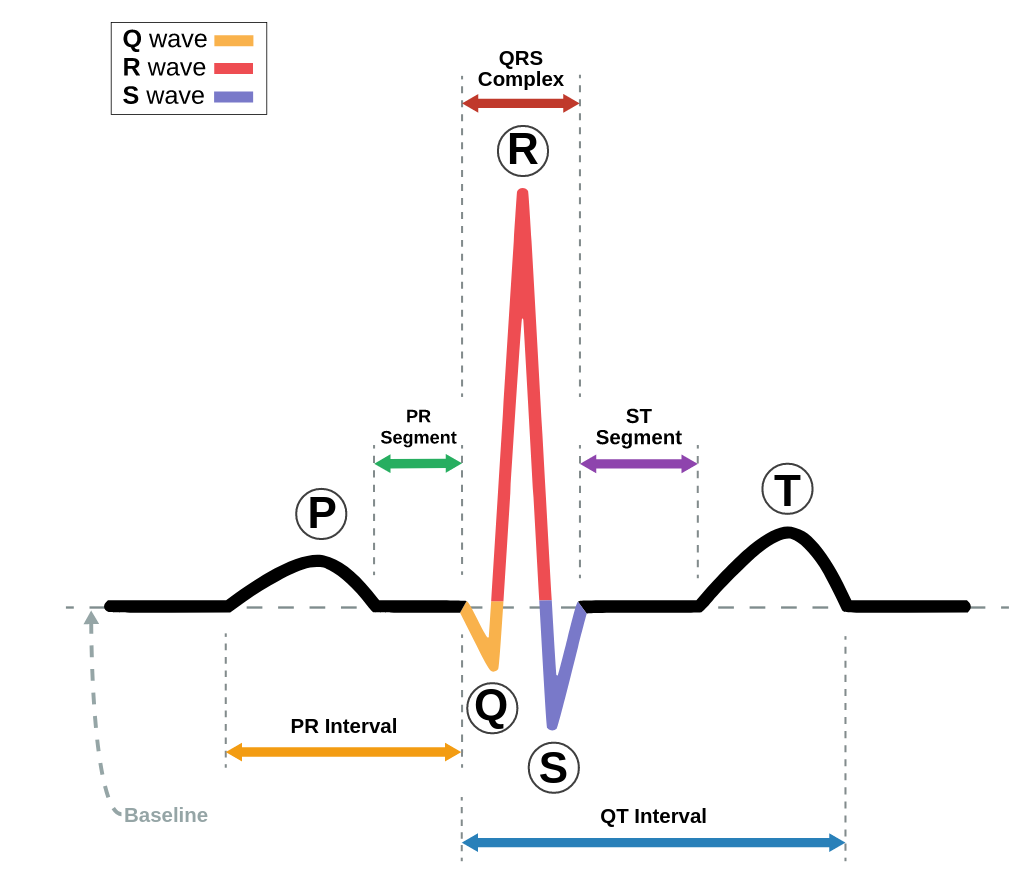
\includegraphics[scale=0.3]{SinusRhythmLabels.png}
    \caption{Schemativ represetation of a regular ECG wave, taken from \href{https://en.wikipedia.org/wiki/QRS_complex}{wikipedia}}
\end{figure}


\begin{figure}[h]
    \centering
    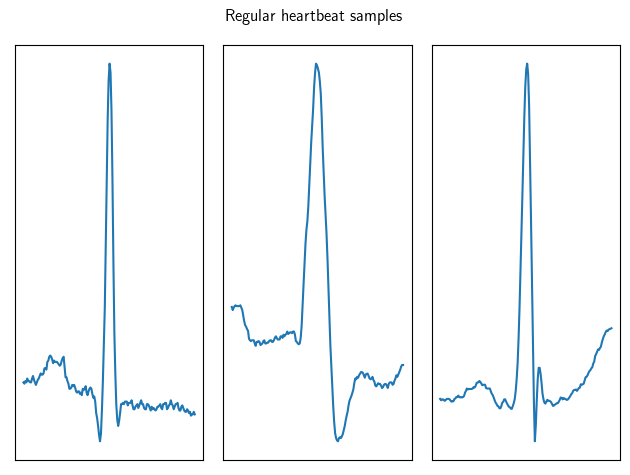
\includegraphics[scale=0.5]{reg_hb_samples.png}
    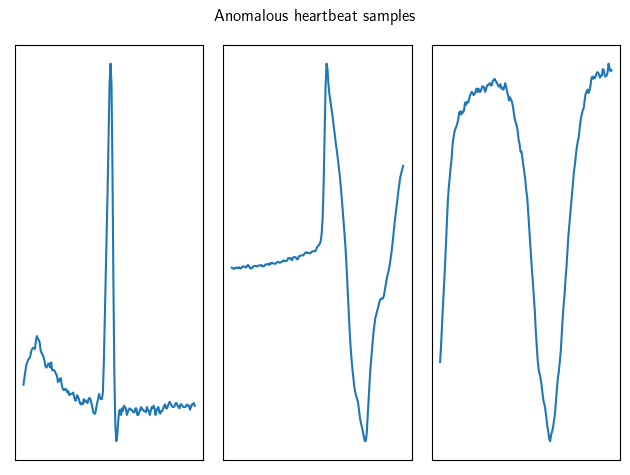
\includegraphics[scale=0.5]{anom_hb_samples.png}
    \caption{Regular and anomalous heart beat samples}
\end{figure}

Before we proceed with the training, we need to preprocess the data. Firstly, since the information contained in both channels are identical, one channel is discarded. We are roughly following the steps from \colorbox{red}{???REF}. This involves normalising the data and extracting single heartbeats from the sequence. To this end, we employ the QRS detector that can detect the R peaks. This is already implemented in the \texttt{wfdb} \parencite{wfdb} package for \texttt{python}. Then, from every peak we consider 90 time steps before and after that peak. This gives one heartbeat with sequence length 180. The associated beat type can then be extracted from the labelled data set. In total this gives over 100 000 single heartbeats each of length 180. We will refer to those samples as private data samples, of which we aim to protect the privacy. In contrast, the generated synthetic data samples will be called public data samples, that we can publish for public use with some associated privacy measure (the privacy is measured by the privacy budget given by the \(\epsilon\) parameter from \cref{def:dp}).

To ensure consistency of results and subsequent comparison of the different model, we split the original data into:
\begin{itemize}
    \item a private training set that consists only of regular samples
    \item a private validation set that consists of roughly equal parts regular and anomalous samples
    \item a private test set that consists of roughly equal parts regular and anomalous samples
\end{itemize}

Therefore, we use the following proportions:

\begin{figure}[H]
    \centering
    \begin{tikzpicture}[
        level 1/.style={sibling distance=5.5cm},
        level 2/.style={sibling distance=2.5cm},
        edge from parent/.style={draw, -, font=\footnotesize, text=gray}, % Adjust font size and color here
        level distance=2.5cm,
        every node/.style={text width=2cm, align=center}, % Add this line for text width and alignment
        boxed/.style={draw, inner sep=3pt}, % Add this style for the box
    ]
    \node (total) {Total: 106008}
      child {node[boxed] {Normal: \\ 87968}
        child {node {86208}
          child {node[boxed] {Train: \\ 69828} edge from parent node[left] {0.81}}
          child {node[boxed] {Validation: \\ 16380} edge from parent node[right, outer sep=-2pt] {0.19}} % Adjust outer sep
          edge from parent node[left] {0.98}
        }
        child {node[boxed] {Test: \\ 1760} edge from parent node[right] {0.02}}
      }
      child {node[boxed] {Anomalous: \\ 18040}
        child {node[boxed] {Test: \\ 1804} edge from parent node[left] {0.1}}
        child {node[boxed] {Validation: \\ 16236} edge from parent node[right] {0.9}}
      };
    
    % Add a rectangular box around the "Total" node and the "Anomalous" node
    \node[fit=(total), draw, inner sep=1pt] {};
    \end{tikzpicture}
    \caption{Division of the private data set into training, test and validation set}
\end{figure}


All preprocessing tasks and subsequent models are implemented in \texttt{python 3.10} on a machine running Arch Linux with kernel version 6.7.4 with 16 GB of RAM, an Nvidia RTX 3070 8GB, and AMD 7700 processor with 8 cores / 16 threads.

\subsection{Baseline Model}
We will establish a baseline model for arrhythmia detection based on an anomaly detection approach from machine learning. One could treat this also a binary classification problem, but due to the class imbalancy, this would decrease the performance. Hence we are following another idea: one popular solution is to train an autoencoder model on only the regular heartbeats. This way, the model is able to compress regular heartbeat sequence into a latent space and recover them with low reconstruction error. When seeing an anomalous sample, the model fails at properly reconstructing the sample, resulting in a high reconstruction error. We will adjust this error threshold using the validation set, that consists of roughly equal numbers of regular and anomalous samples.

The baseline model is an LSTM-autoencoder with two components:
\begin{itemize}
    \item \underline{Encoder component:} The encoder takes in the one-dimensional heartbeat sequence. There are two LSTM layers that encode the sequence into a latent space. We fixed the dimension of the latent space to 32.
    \item \underline{Decoder component:} The decoder works similar to the encoder but the other way around. Hence, we design it to take in an encoded vector representation of the heartbeat sequence in the latent space with dimension 32 and output a heartbeat sequence one time step after the other.
\end{itemize}

\begin{figure}[h]
    \centering
    \resizebox{0.5\textwidth}{!}{%
    \begin{circuitikz}
    \tikzstyle{every node}=[font=\Large]
    \draw [](6.25,15.5) to[short] (17.5,15.5);
    \draw (6.25,15.5) to[short] (17.5,15.5);
    \draw [](7.5,10.5) to[short] (16.25,10.5);
    \draw [short] (6.25,15.5) -- (7.5,10.5);
    \draw [short] (16.25,10.5) -- (17.5,15.5);
    \draw [](6.25,-2) to[short] (17.5,-2);
    \draw (6.25,15.5) to[short] (17.5,15.5);
    \draw [](7.5,3) to[short] (16.25,3);
    \draw [short] (16.25,3) -- (17.5,-2);
    \draw [short] (6.25,-2) -- (7.5,3);
    \node [font=\LARGE] at (8,15) {Encoder};
    \node [font=\LARGE] at (14.5,2.25) {Decoder};
    \draw [ color={rgb,255:red,94; green,92; blue,100} , dashed] (12,18.25) ellipse (7.75cm and 1cm);
    \node [font=\large] at (11.75,18.25) {Original heartbeats};
    \draw [->, >=Stealth] (12,17) .. controls (12,16.75) and (12,16.5) .. (12,15.75) ;
    \draw [ color={rgb,255:red,94; green,92; blue,100} , dashed] (11.75,-4.75) ellipse (7.75cm and 1cm);
    \node [font=\large] at (11.5,-4.75) {Generated heartbeats};
    \draw [->, >=Stealth] (11.5,-8.5) .. controls (11.5,-9) and (11.5,-9) .. (11.5,-9.75) ;
    \draw  (4,6.75) circle (0.75cm) node {\LARGE $l_1$} ;
    \draw  (6.25,6.75) circle (0.75cm) node {\LARGE $l_2$} ;
    \draw  (8.5,6.75) circle (0.75cm) node {\LARGE $l_3$} ;
    \node [font=\huge] at (13.25,7) {. . . . . . . . . . . . . . . . . . };
    \draw  (17.5,6.75) circle (0.75cm) node {\LARGE $l_{d-1}$} ;
    \draw  (20,6.75) circle (0.75cm) node {\LARGE $l_d$} ;
    \draw  (8.75,13.75) circle (0.5cm) node {\LARGE $s_1$} ;
    \draw  (8,12.75) rectangle  node {\normalsize LSTM} (9.75,11.5);
    \draw  (10.75,12.75) rectangle  node {\normalsize LSTM} (12.5,11.5);
    \draw  (11.5,13.75) circle (0.5cm) node {\LARGE $s_2$} ;
    \draw  (14.5,12.75) rectangle  node {\normalsize LSTM} (16.25,11.5);
    \draw  (15.25,13.75) circle (0.5cm) node {\LARGE $s_n$} ;
    \node [font=\huge] at (13.75,12.25) {. . . };
    \draw [->, >=Stealth] (9.75,12) -- (10.75,12);
    \draw [->, >=Stealth] (15.5,11.5) -- (15.5,8.5);
    \draw [->, >=Stealth] (8.5,5.5) -- (8.5,1.25);
    \draw  (7.75,-0.25) rectangle  node {\normalsize LSTM} (9.5,-1.5);
    \draw  (8.5,0.75) circle (0.5cm) node {\LARGE $l_1$} ;
    \draw [->, >=Stealth] (9.5,-1) -- (10.5,-1);
    \draw  (10.5,-0.25) rectangle  node {\normalsize LSTM} (12.25,-1.5);
    \draw  (11.25,0.75) circle (0.5cm) node {\LARGE $l_2$} ;
    \node [font=\huge] at (13.5,-0.75) {. . . };
    \draw  (14.25,-0.25) rectangle  node {\normalsize LSTM} (16,-1.5);
    \draw  (15,0.75) circle (0.5cm) node {\LARGE $l_d$} ;
    \draw [->, >=Stealth] (15.25,-1.5) -- (15.25,-4.5);
    \draw [->, >=Stealth, dashed] (12.25,-1) -- (14.25,-1);
    \draw [->, >=Stealth, dashed] (12.5,12) -- (14.5,12);
    \draw [->, >=Stealth] (8.75,13.25) -- (8.75,12.75);
    \draw [->, >=Stealth] (8.5,0.25) -- (8.5,-0.25);
    \draw [->, >=Stealth] (11.25,0.25) -- (11.25,-0.25);
    \draw [->, >=Stealth] (15,0.25) -- (15,-0.25);
    \draw [->, >=Stealth] (11.5,13.25) -- (11.5,12.75);
    \draw [->, >=Stealth] (15.25,13.25) -- (15.25,12.75);
    \draw [, dashed] (2.25,9.25) rectangle  (21.25,4.25);
    \node [font=\Large] at (4,8.75) {Latent space};
    \end{circuitikz}
    }%
    
    \label{fig:my_label}
    \caption{Architecture of baseline model}
    \end{figure}

\subsubsection*{Training the Baseline Model}
We train the model on the training set which consists of roughly 70 000 regular heartbeat samples. As loss function we take the mean-squared-error (MSE) between original and reconstructed sample. Training is done using the Adam optimiser with learning rate 5e-4, $\beta_1=0.9$ and $\beta_2=0.999$ for 20 epochs with batch size 1. As we can see from \cref{fig:loss_baseline}, the loss function converges well indicating a (locally) optimal solution with an average reconstruction error slightly below 1. The loss for the validation set decreases similarly with the training error. This indicates that the model can generalise well to unseen regular heartbeat data.

\begin{figure}[h]
    \centering
    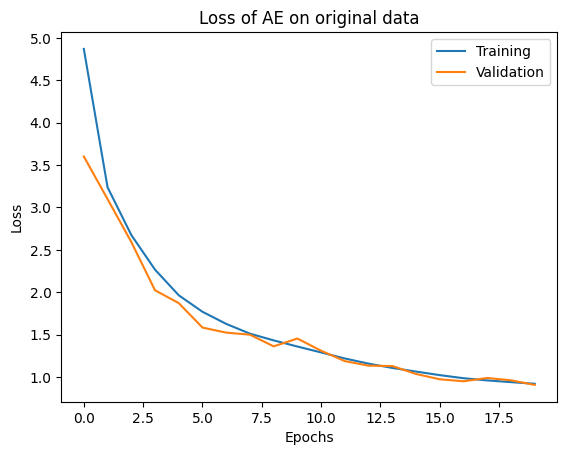
\includegraphics[scale=0.7]{loss_baseline.png}
    \caption{Loss over epoch for baseline model together with loss on validation set}
    \label{fig:loss_baseline}
\end{figure}

When inputting a regular test sample, the model seems to capture all the visually important features and even removes some of the underlying noise.

\begin{figure}[H]
    \centering
    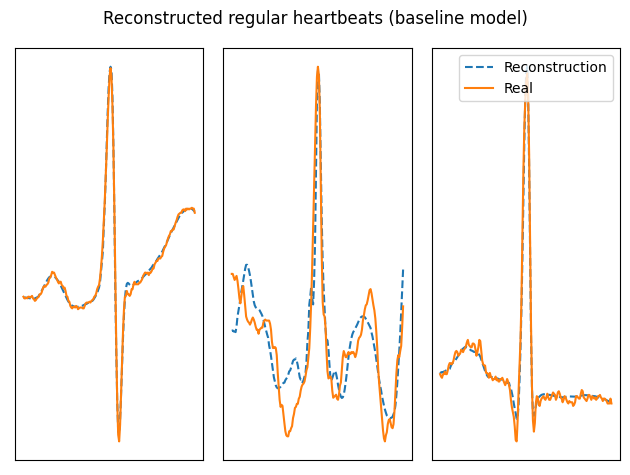
\includegraphics[scale=0.7]{rec_reguarl_samples_baseline.png}
    \caption{Regular test sample vs. reconstructed sample}
    \label{fig:regog_vs_recon}
\end{figure}

Now we do the same but with an anomalous sample for demonstration purposes as can be seen in \cref{fig:anomog_vs_recon}.

\begin{figure}[h]
    \centering
    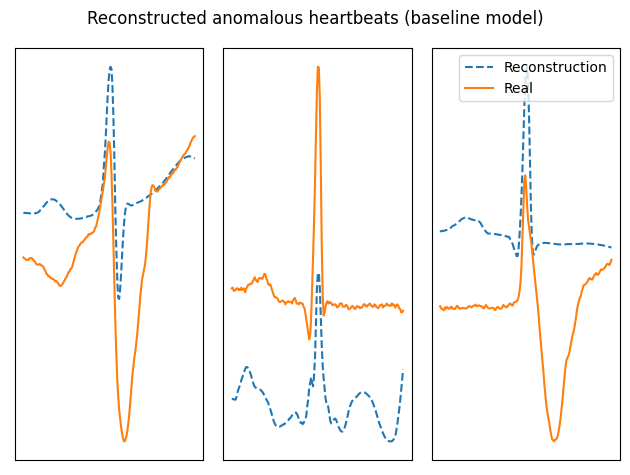
\includegraphics[scale=0.7]{rec_anom_samples_baseline.png}
    \caption{Anomalous test sample vs. reconstructed sample}
    \label{fig:anomog_vs_recon}
\end{figure}

\subsubsection*{Performance of baseline model}
So visually, we can already verify that the baseline model seems to be able to distinguish between regular and anomalous samples. We now find an optimal threshold for the reconstruction error and measure the performance. Using the determined theshold value, we do the classification as follows: we input a sample to the anomaly detection model, which outputs the reconstructed sample with some error. If the error is below the threshold, it will be classified as a regular heartbeat, otherwise it will be classified as an anomalous heartbeat. Firstly, let us plot the error distribution the held out validation set:

\begin{figure}[H]
    \centering
    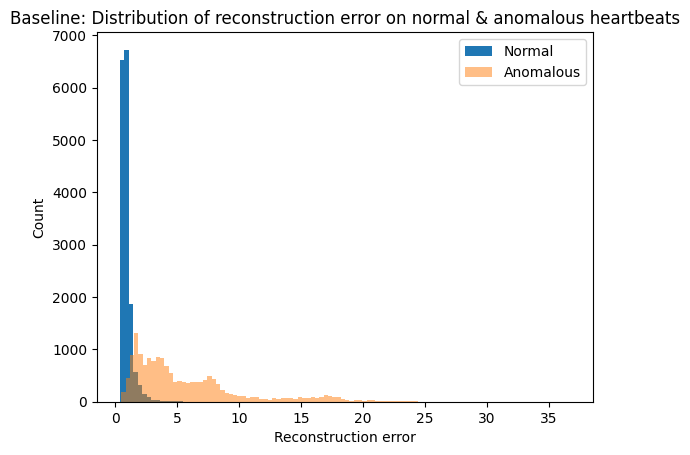
\includegraphics[scale=0.7]{hist_threshold_baseline.png}
    \caption{Distribution of reconstruction error for regular and anomalous samples in the validation set.}\label{fig:distr_err_baseline}
\end{figure}
Clearly, the average error is much lower for regular heartbeats. Thus, the model is able to distinguish regular from anomalous samples by reconstruction error. We can find the ``good'' threshold for the error by computing the percentage of correctly classified regular samples and correctly classified anomalous samples based on different threshold values. From \cref{fig:thres_baseline} we can see that the percentage of correctly classified regular samples slowly increases, while the percentage of correctly classfied anomalous samples decreases. This is to be expected, since a threshold value of 0 would simply classify all samples as anomalous, giving perfect classification for anomalous samples. Conversely, a very high threshold value (e. g. 20) would tend to classify each samples as regular, yielding perfect classification for regular samples. We need to strike a balance between those two extremes by examining \cref{fig:thres_baseline}.

\begin{figure}[h]
    \centering
    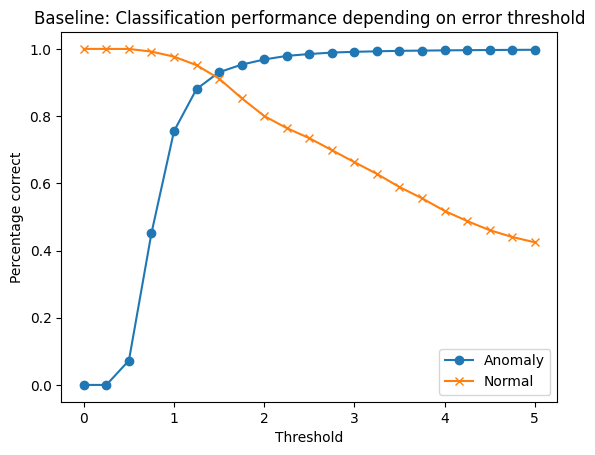
\includegraphics[scale=0.7]{thres_plot_baseline.png}
    \caption{Percentages of correctly classified samples based on different threshold values}
    \label{fig:thres_baseline}
\end{figure}

There are different ways to find a well-suited threshold depending on whether one want to have better performance on anomalous or regular samples. We choose to not favour any classification over the other, hence the neutral decision strategy for the threshold value is the one where both lines cross. Choosing the threshold here to be 1.5, we can compute different metrics that measure the performance of the arrhythmia detection (where TN=True Negatives, TP=True Positives, FN=False Negatives, FP=False Positives):

\begin{itemize}
    \item Accuracy measures the overall percentage of correct classifications:
    \begin{align}
        Accuracy = \frac{TP+TN}{TP+FP+TN+FN}
    \end{align}
    \item Precision looks only on the samples that are labelled as anomalies and computes the percentages of correctly detected anomalies:
    \begin{align}
        Precision = \frac{TP}{TP+FP}
    \end{align}
    \item Recall looks at all true anomalies and computes the percentage of correctly detected anomalies
    \begin{align}
        Recall = \frac{TP}{TP+FN}
    \end{align}
    \item F1 computes the an average of Precision and Recall
    \begin{align}
        F1 = \frac{2\cdot Precision\cdot Recall}{Precision + Recall}
    \end{align}
\end{itemize}

\subsubsection*{Summary of performance evaluation}
Since we will reuse the previous performance evaluation procedure for measuring the utility of the generated data, we quickly summarise the process:
\begin{enumerate} \label{list:anom_eval}
    \item Train an autoencoder on the synthetic training data set consisting of only regular samples. This synthetic training data is generated by our two different models.
    \item Based on the distribution of the reconstruction errors on the private validation set for regular and anomalous samples, we determine a threshold value for classification.
    \item We evaluate the utility of the generated data based on metrics for anomaly detection.
\end{enumerate}

This approach commonly referred to as the ``Train on synthetic, test on real'' (TSTR) paradigm \parencite{esteban2017realvalued} that is being used to measure utility of synthetic data.

\subsection{Data generation}
Now we use the models presented in \cref{chapter4} to generate some synthetic heartbeat data. We will train the models on the private training data set, that consists only of regular samples. In turn, the models should be able to generate only regular heartbeat samples. Since both models are similar in architecture, the training procedure can be jointly described:
\begin{enumerate}
    \item We train the autoencoder module separately from rather than jointly with the generator. The authors in \parencite{pei2021towards} have found that there is no significant performance improvement when training jointly. This means, the models first learn how to encode the heartbeat time series in a shared latent space and how to decode it back from it. Conveniently, this is exactly the same autoencoder that is being used by the baseline model for arrhythmia detection, so we do not need to train it again.
    \item We train the generator on encoded training data, i. e. we pass the private training data to the encoder which returns an encoded version of that training data in the latent representation. Then the generator trains to generate this latent representation.
    \item After training, the generator generates a synthetic training set with the same number of samples as the private training set.
    \item We evaluate the utility of the synthetic data by measuring its performance on anomaly detection following the procedure described in \cref{list:anom_eval}.
\end{enumerate}

\subsubsection*{AE-MERF}
We train the AE-MERF model with the following configuration:
\begin{table}[H]
    \centering
    \begin{tabular}{|c|c|c|}
        \hline
        \multirow{4}{*}{\textbf{Autoencoder}}& Embedding dimension & 32 \\ 
                                    & Learning rate & 5e-4 \\
                                    & Number of epochs& 20\\
                                    & Batch size & 1\\
        \hline
        \multirow{4}{*}{\textbf{Generator (MERF)}} & Number of random features & 2000 \\
                                        & Learning rate & 1e-3\\
                                        & Number of epochs & 20\\
                                        & Batch Size & 7000 \\
        \hline
    \end{tabular}
    \caption{Configuration for AE-MERF}
\end{table}
We then let the model generate some training samples: 

\begin{figure}[h]
    \centering
    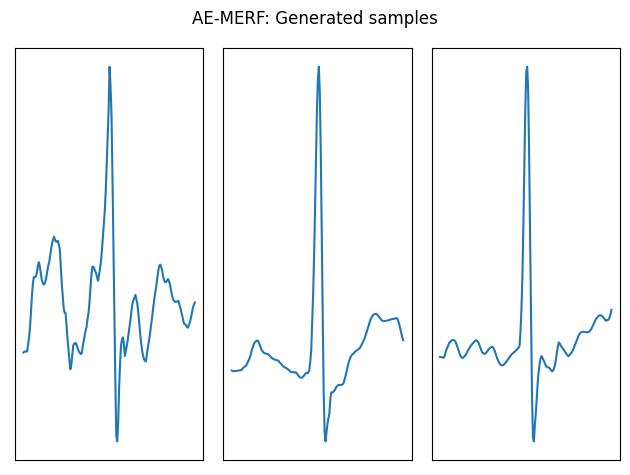
\includegraphics[scale=0.7]{gen_aemerf.png}
    \caption{Generated regular heartbeats by AE-MERF model}
\end{figure}

To assess the utility, we now train an anomaly detection model with a synthetic training data set. Therefore, we generate a synthetic data set with the same number of samples as the original private training data set, i. e. roughly 70 000 regular heart beat samples. We use the same architecture as for the baseline model - an LSTM autoencoder with embedding dimesion 32. As we can see from the loss in \cref{fig:loss_aemerf}, the model converges on the synthetic training data, while still being able to generalise on the private validation set (that contains real-life samples). The error on the validation set is abit higher though in contrast to the baseline model. The training loss is again slightly below 1 while the validation loss averages around 2. 

\begin{figure}[h]
    \centering
    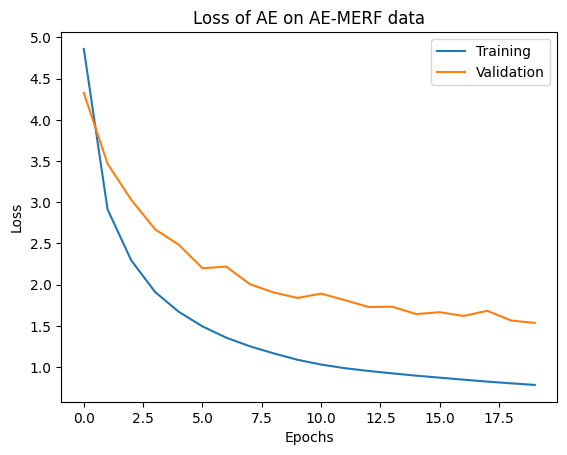
\includegraphics[scale=0.7]{loss_aemerf.png}
    \caption{Loss over epoch for baseline model together with loss on validation set}
    \label{fig:loss_aemerf}
\end{figure}

Now following the established methodology, we compute a good threshold based on which we can distinguish between regular and anomalous samples:

\begin{figure}[h]
    \begin{minipage}[b]{0.45\textwidth}
        \centering
        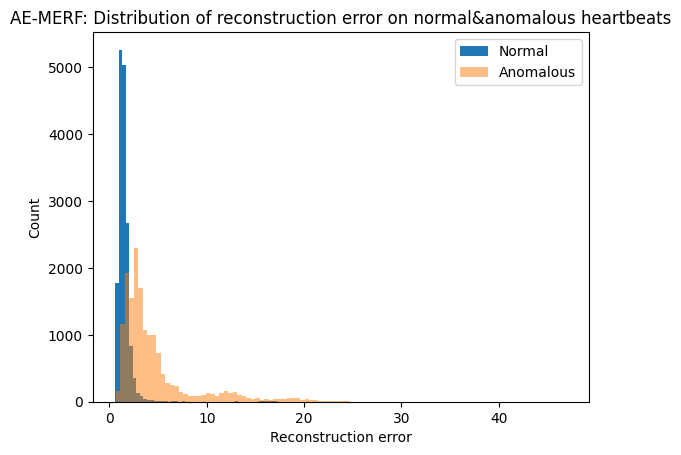
\includegraphics[scale=0.4]{hist_threshold_aemerf.png}
        \caption{Caption}
        \label{fig:enter-label}
    \end{minipage}
    \begin{minipage}[b]{0.45\textwidth}
        \centering
        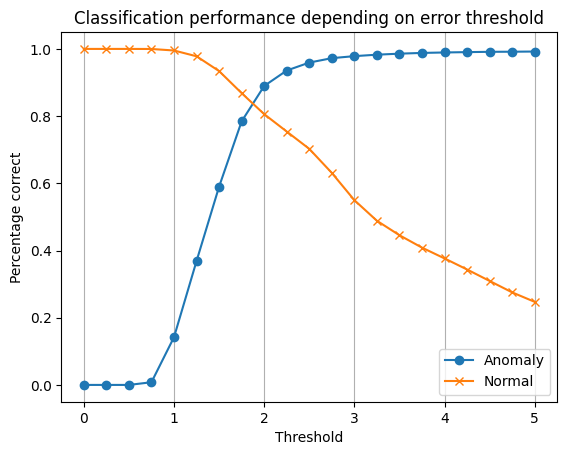
\includegraphics[scale=0.4]{thres_plot_aemerf.png}
        \caption{Caption}
        \label{fig:enter-label}
    \end{minipage}
\end{figure}

This gives an error threshold of 1.75. This is slighty higher than threshold computed for the baseline model trained on private data, which indicates that the generator introduced some errors.

\subsubsection*{AE-WGAN}
We train the AE-WGAN model with the following configuration:

\begin{table}[h]
    \centering
    \begin{tabular}{|c|c|c|}
        \hline
        \multirow{4}{*}{\textbf{Autoencoder}}& Embedding dimension & 32 \\ 
                                    & Learning rate & 5e-4 \\
                                    & Number of epochs& 20\\
                                    & Batch size & 1\\
        \hline
        \multirow{4}{*}{\textbf{Generator (WGAN)}} & Discriminator steps & 3 \\
                                        & Learning rate & 9e-3\\
                                        & Number of iterations & 15000\\
                                        & Batch Size & 256 \\
        \hline
    \end{tabular}
    \caption{Configuration for AE-WGAN}
\end{table}

Again, we let the model generates some regular heartbeat samples:
\begin{figure}[H]
    \centering
    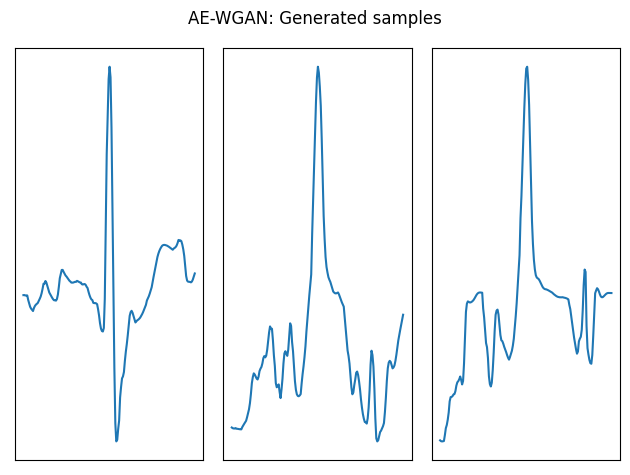
\includegraphics[scale=0.7]{gen_aewgan.png}
    \caption{Generated regular heartbeats by AE-WGAN model}
\end{figure}

Compared to the generated samples from the AE-MERF model, the AE-WGAN model generates samples appear to be much noisier. We expect that the reconstruction error for the arrhythmia detection task will then also be much higher. We again train an LSTM-autoencoder on the synthetic training data generated by AE-WGAN. Looking at the loss, we can see that the validation error is much higher than the training error now. This leads to the assumption, that the generated samples differ quite much from the true samples, while still maintaining some important characteristics as the validation is also slowly decreasing.

\begin{figure}[H]
    \centering
    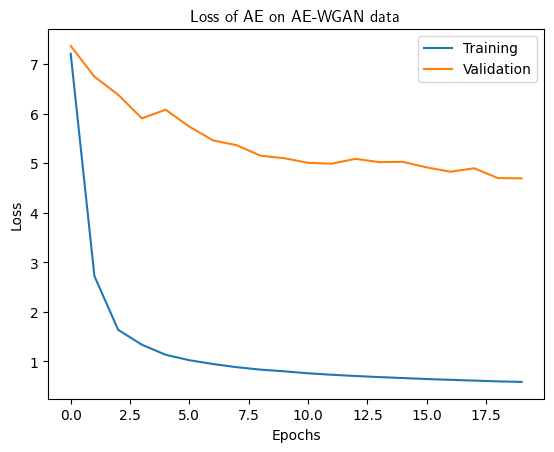
\includegraphics[scale=0.7]{loss_aegwan.png}
    \caption{Loss over epoch for AE-WGAN model together with loss on validation set}
\end{figure}

This behaviour is mirrored when finding the threshold for anomaly detection:
\begin{figure}[h]
    \begin{minipage}[b]{0.45\textwidth}
        \centering
        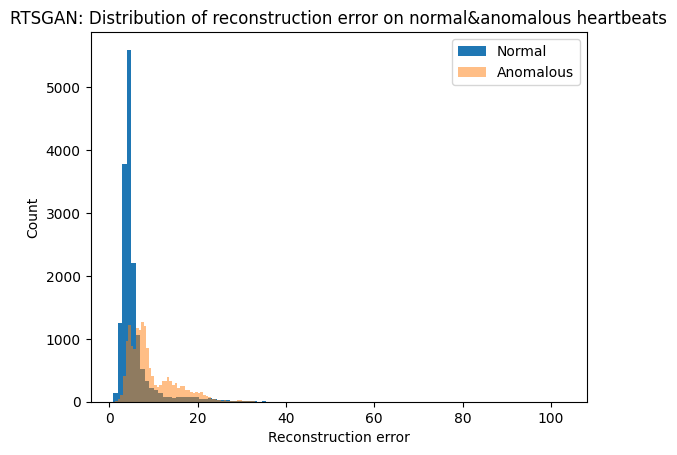
\includegraphics[scale=0.4]{hist_threshold_aewgan.png}
        \caption{Caption}
        \label{fig:enter-label}
    \end{minipage}
    \begin{minipage}[b]{0.45\textwidth}
        \centering
        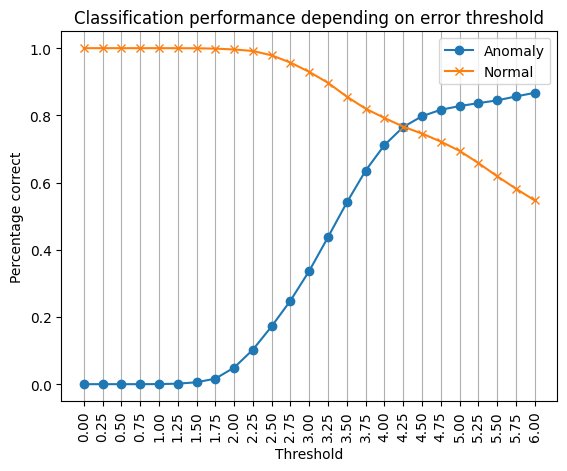
\includegraphics[scale=0.4]{thres_plot_aewgan.png}
        \caption{Caption}
        \label{fig:enter-label}
    \end{minipage}
\end{figure}

The threshold is much higher now, which again confirms the fact, that the samples generated by AE-WGAN deviate much more from the original samples.

\subsection{Privacy-preserving Data Generation}
We now follow the same procedure as previously but add DP noise to each model. How noise is calibrated and added is described in \cref{chapter4}. We follow the same TSTR methodology as with the non-privacy-preserving models. For ease of reading, we omit the plots from training for now and refer to the appendix if needed. 

\subsubsection*{AE-dpMERF}
We use the DP version AE-dpMERF to generate some samples with DP guarantees. In particular, we generate samples with $\epsilon=1, 0.5, 0.01, 0.001$ and assess their utility for anomaly detection.

\begin{figure}[H]
    \centering
    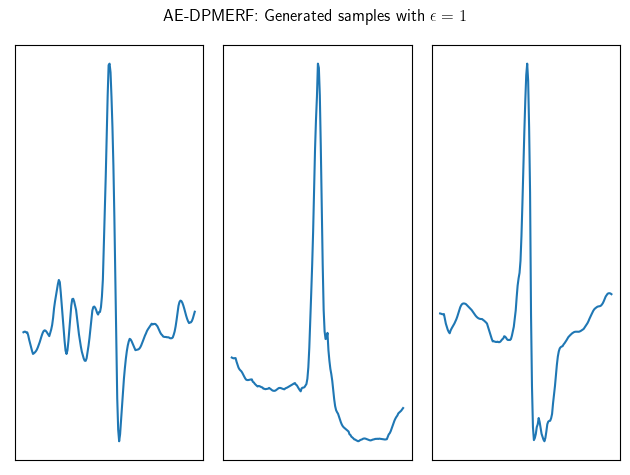
\includegraphics[scale=0.5]{gen_aedpmerf_eps1.png}
    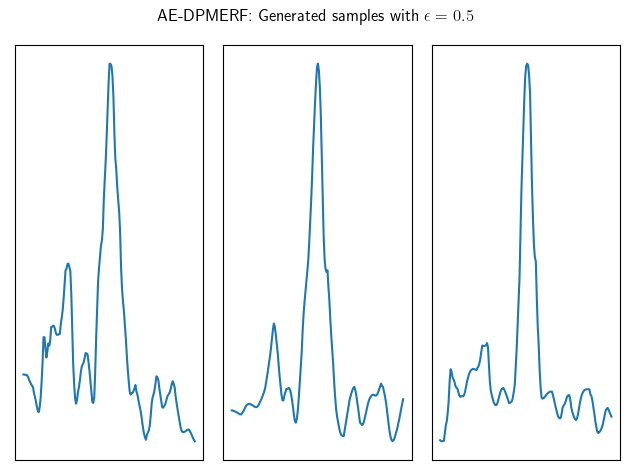
\includegraphics[scale=0.5]{gen_aedpmerf_eps05.png}
    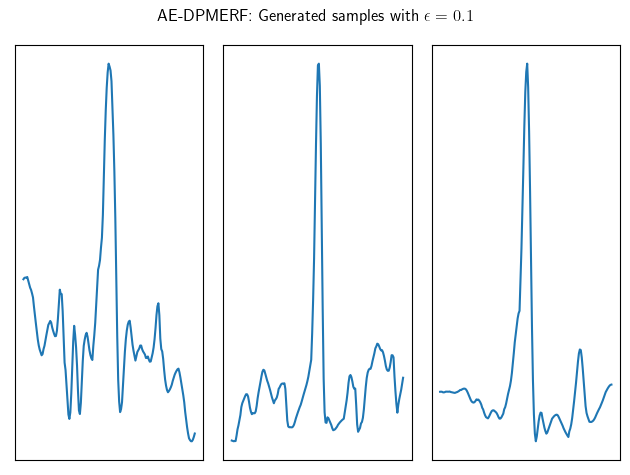
\includegraphics[scale=0.5]{gen_aedpmerf_eps01.png}
    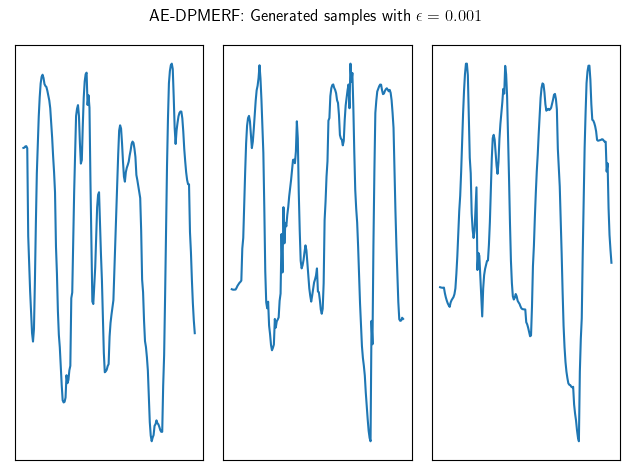
\includegraphics[scale=0.5]{gen_aedpmerf_eps001.png}
    \caption{AE-dpMERF generated samples with different $\epsilon$, the lower the value the higher the privacy guarantees}
    \label{fig:gen_aedpmerf}
\end{figure}

As we can see, the lower the $\epsilon$ privacy parameter the more noise is introduced. This gives stricter privacy guarantees, but for $\epsilon=0.001$ too much noise is added and the generated samples visually do not appear to show a regular heartbeat. Clearly we can see from the generated samples in \cref{fig:gen_aedpmerf}, that more noise during training also results in more noise for the generated samples.  In practice, it is recommended to use an $\epsilon$ value of 1, so AE-dpMERF with $\epsilon=1$ already gives visually satisfying results \parencite{dwork2019differential}.

\subsubsection*{AE-dpWGAN}
We use the DP version AE-dpWGAN to generate some samples with DP guarantees and $\epsilon=35, 25, 5$. As the training for GANs is inherently very unstable and therefore sensitive to changes, we did not get satisfying results with even lower epsilon values. 

\begin{figure}[H]
    \centering
    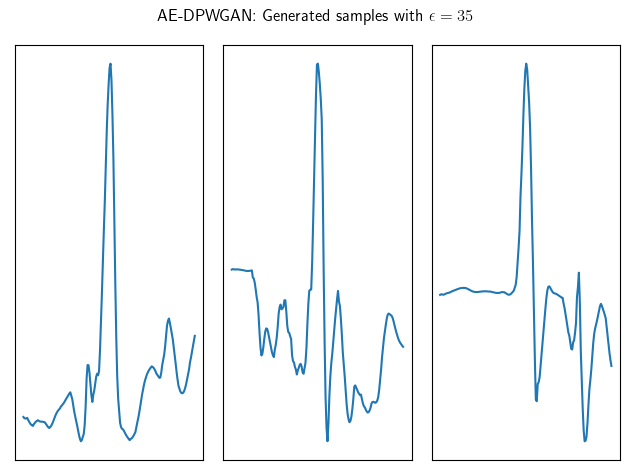
\includegraphics[scale=0.6]{gen_aedpwgan_eps35.png}
    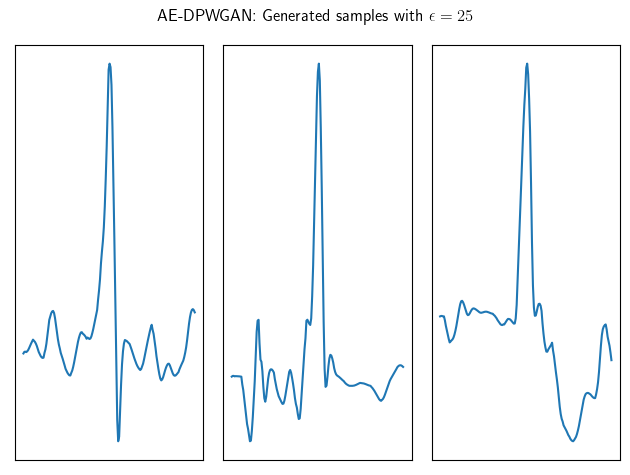
\includegraphics[scale=0.6]{gen_aedpwgan_eps25.png}
    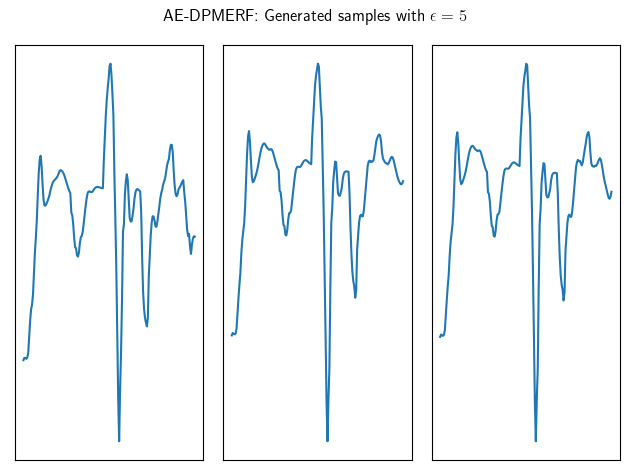
\includegraphics[scale=0.6]{gen_aedpwgan_eps5.png}
    \caption{AE-dpWGAN generated samples with different $\epsilon$, the lower the value the higher the privacy guarantees}
    \label{fig:enter-label}
\end{figure}

As we can see, even with $\epsilon=35$ there is a lot of visible noise in the generated samples. This behaviour gets worse with decreasing $\epsilon$. When training with $\epsilon=5$ too much noise is added and the GAN gets really hard to train properly. 

\subsection{Results}
We are now ready to compare all the different models in terms of their performance on anomaly detection. \cref{tab:results} shows a summary of all models in their performance scores. We also summarise this information in \cref{fig:res_aedpmerf}. It is apparent that utility is lost already during (non-privacy-preserving) data generation. The loss in utility is around 10\% for AE-MERF and 15\% for AE-WGAN. Additionally, surprisingly we see that their is no significant loss in utility when introducing differential privacy to either models up to a certain $\epsilon$ value. For AE-dpMERF with $\epsilon=0.5, 1$ the recall value is even higher than for the baseline model. Of course, the generated samples contain much more noise, thus leading to higher reconstruction error as we have seen before, but this does not impact the anomaly detection performance too much. Once the $\epsilon$ value is too low, thus too much noise is added during generation, the generated samples loose their utility for anomaly detection. For AE-dpMERF the lowest observed value is $\epsilon=0.5$ for which we do not see a decrease in utility. On the other, synthetic samples generated by AE-dpWGAN become too noisy already with much higher $\epsilon$ values, e. g. $\epsilon=5$. 
\begin{table}[h]
    \centering
    \begin{tabular}{c||c|c|c|c}
        Model & Accuracy & Precision & Recall & F1 \\ 
        \hline 
        \hline

        Baseline & 0.92 & 0.91 & 0.94 & 0.92 \vspace{0.5cm}\\
        \hline

        AE-MERF & 0.83 & 0.85 & 0.79 & 0.82 \\
        \hline
        AE-DPMERF ($\epsilon=1$) & 0.83 & 0.81 & 0.86 & 0.83 \\
        \hline
        AE-DPMERF ($\epsilon=0.5$) & 0.81 & 0.81 & 0.80 & 0.80 \\
        \hline
        AE-DPMERF ($\epsilon=0.1$) & 0.76 & 0.75 & 0.77 & 0.76\\
        \hline
        AE-DPMERF ($\epsilon=0.01$) & 0.48 & 0.47 & 0.41 & 0.43 \vspace{0.5cm}\\
        \hline

        AE-WGAN & 0.76 & 0.75 & 0.75 & 0.75 \\
        \hline
        AE-DPWGAN ($\epsilon=35$) & 0.74 & 0.74 & 0.75 & 0.74 \\
        \hline
        AE-DPWGAN ($\epsilon=25$) & 0.72 & 0.73 & 0.71 & 0.71 \\
        \hline
        AE-DPWGAN ($\epsilon=5$) & 0.56 & 0.56 & 0.57 & 0.56\\

    \end{tabular}
    \caption{Summary of anomaly detection performance}
    \label{tab:results}
\end{table}

\begin{figure}[H]
    \centering
    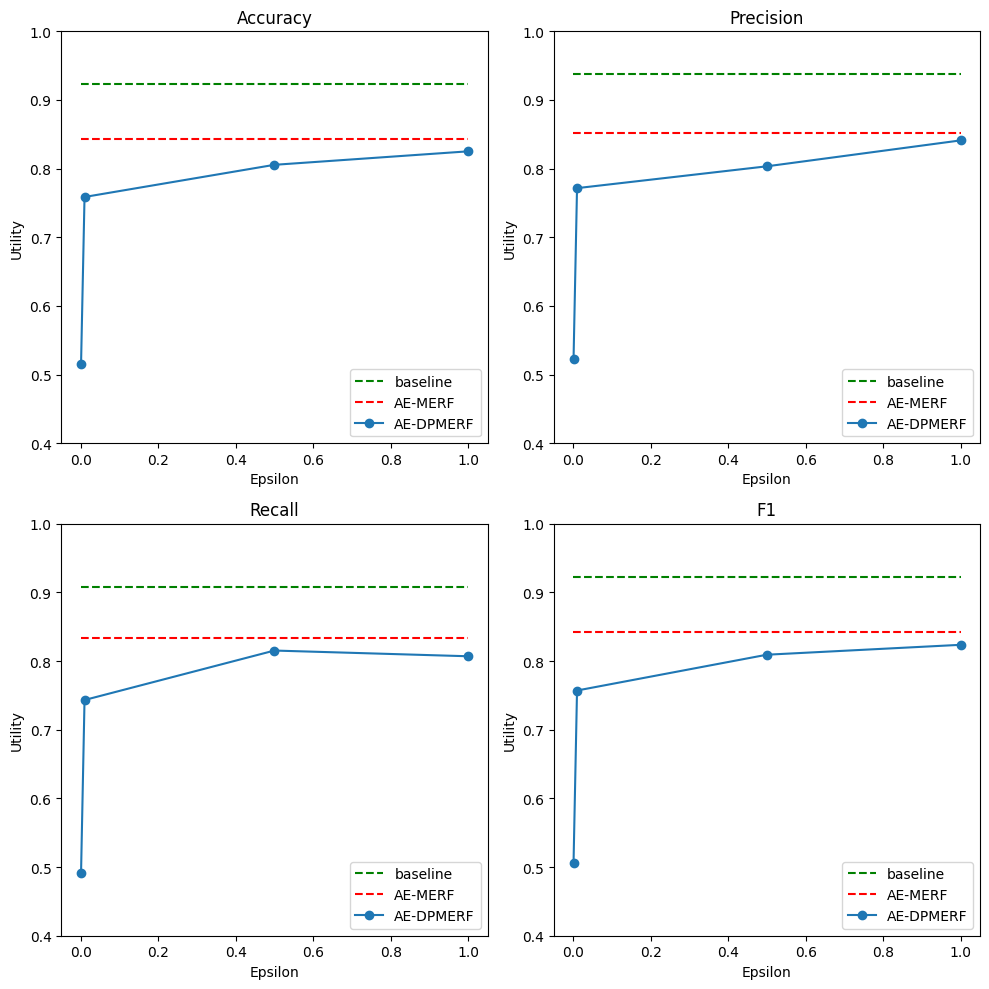
\includegraphics[scale=0.6]{results_aedpmerf.png}
    \caption{Utility loss over privacy budget $\epsilon$ for AE-(dp)MERF}
    \label{fig:res_aedpmerf}
\end{figure}

\begin{figure}[H]
    \centering
    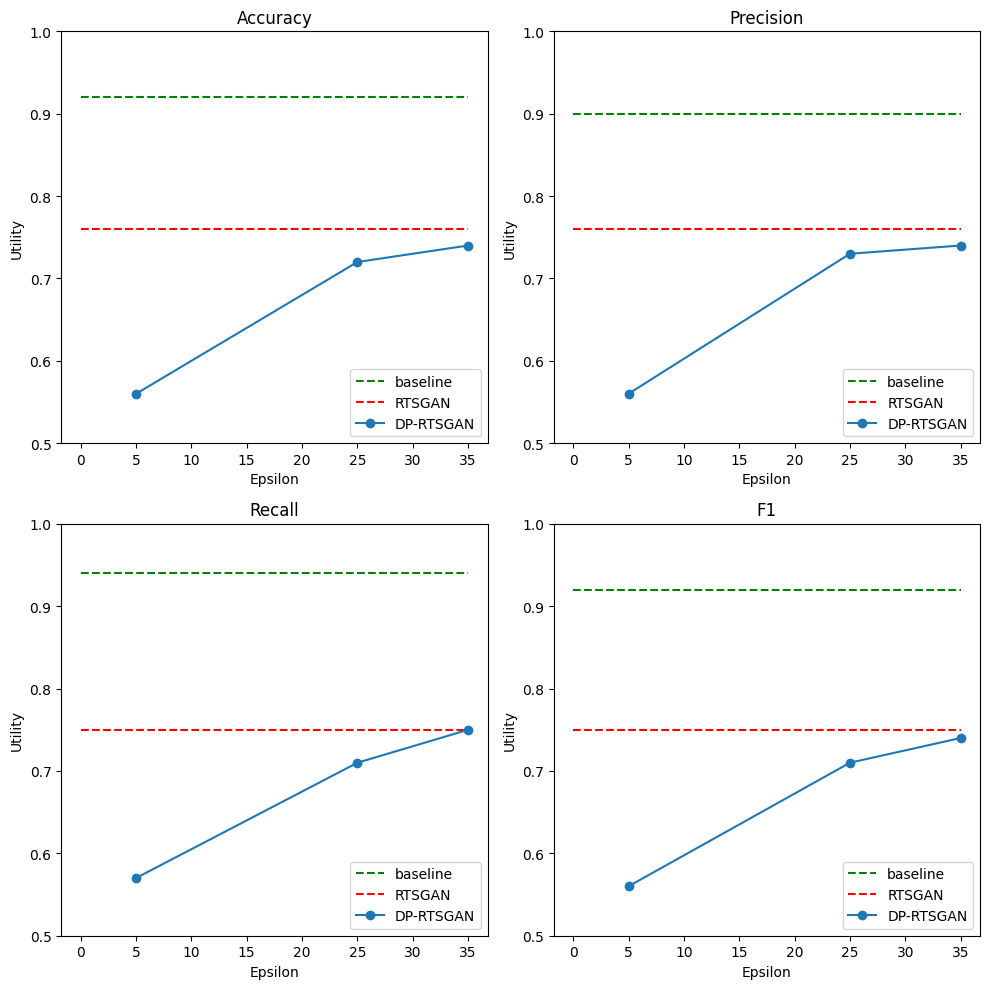
\includegraphics[scale=0.6]{restuls_dprtsgan.png}
    \caption{Utility loss over privacy budget $\epsilon$ for AE-(dp)WGAN}
    \label{fig:res_aedpmerf}
\end{figure}

\subsection{Contaminated Data Set}
Now we contaminate the original training set that previously consisted of regular heartbeat samples only with some anomalous ones. This serves two purposes:
\begin{enumerate}
    \item In real-life, labelled data is rare and heartbeat arrhythmia are scarce (1.5 - 5\%). Having a contaminated training data set can simulate this scenario.
    \item We can check how adding DP to the generation procedure will impact the robustness of the generated samples. 
\end{enumerate}

Therefore, we contaminate the training data with 1\%, 2\% and 5\% of anomalous heartbeat samples and repeat the data generation and anomaly detection as before.